\documentclass[aspectratio=169]{beamer}
\setbeamertemplate{navigation symbols}{}
\usepackage{color,amsmath,comment, subfigure}
\usepackage{booktabs}



%%%%%%%%%%%%%%%%%%%%%%%%%%
\title[]{Lecture 20: Social media and social ads}
\author[]{Matthew J. Salganik}
\institute[]{Sociology 204: Social Networks\\Princeton University}
\date[]{
1/2 Social targeting of ads
\vfill

\begin{flushleft}
\vspace{0.6in}

\includegraphics[width=0.1\textwidth]{figures/cc.png}
\end{flushleft}
}

% Pre-read
% As we think about how social media impacts individuals and society, and how we might fix social media, we need to keep in mind that social media companies are created and run to make money. These are not charities.
% They make money by selling ads, some of which use social data explicitly. In these readings we will understand the ads part of social media in more detail.
% One broad framework to bring to these readings is the idea of surveillance capitalism proposed by Zuboff. Commodification of personal data for profit.
% Duhigg provides a primer on surveillance capitalism and using data for targeting ads
% Goel and Goldstein study when adding in social data improves ad targeting
% Bakshy et al study when adding social information to ad creatives (e.g., endorsements) can impact engagement and how to separate that impact from homophily (the tendency of people to be connect to similar people)
% Goel and Goldstein use observation data and Bakshy et al run experiments.

\begin{document}
%%%%%%%%%%%%%%%%%%%%%%%%%%%
\frame{\titlepage}
%%%%%%%%%%%%%%%%%%%%%%%%%%%
\begin{frame}

\begin{center}
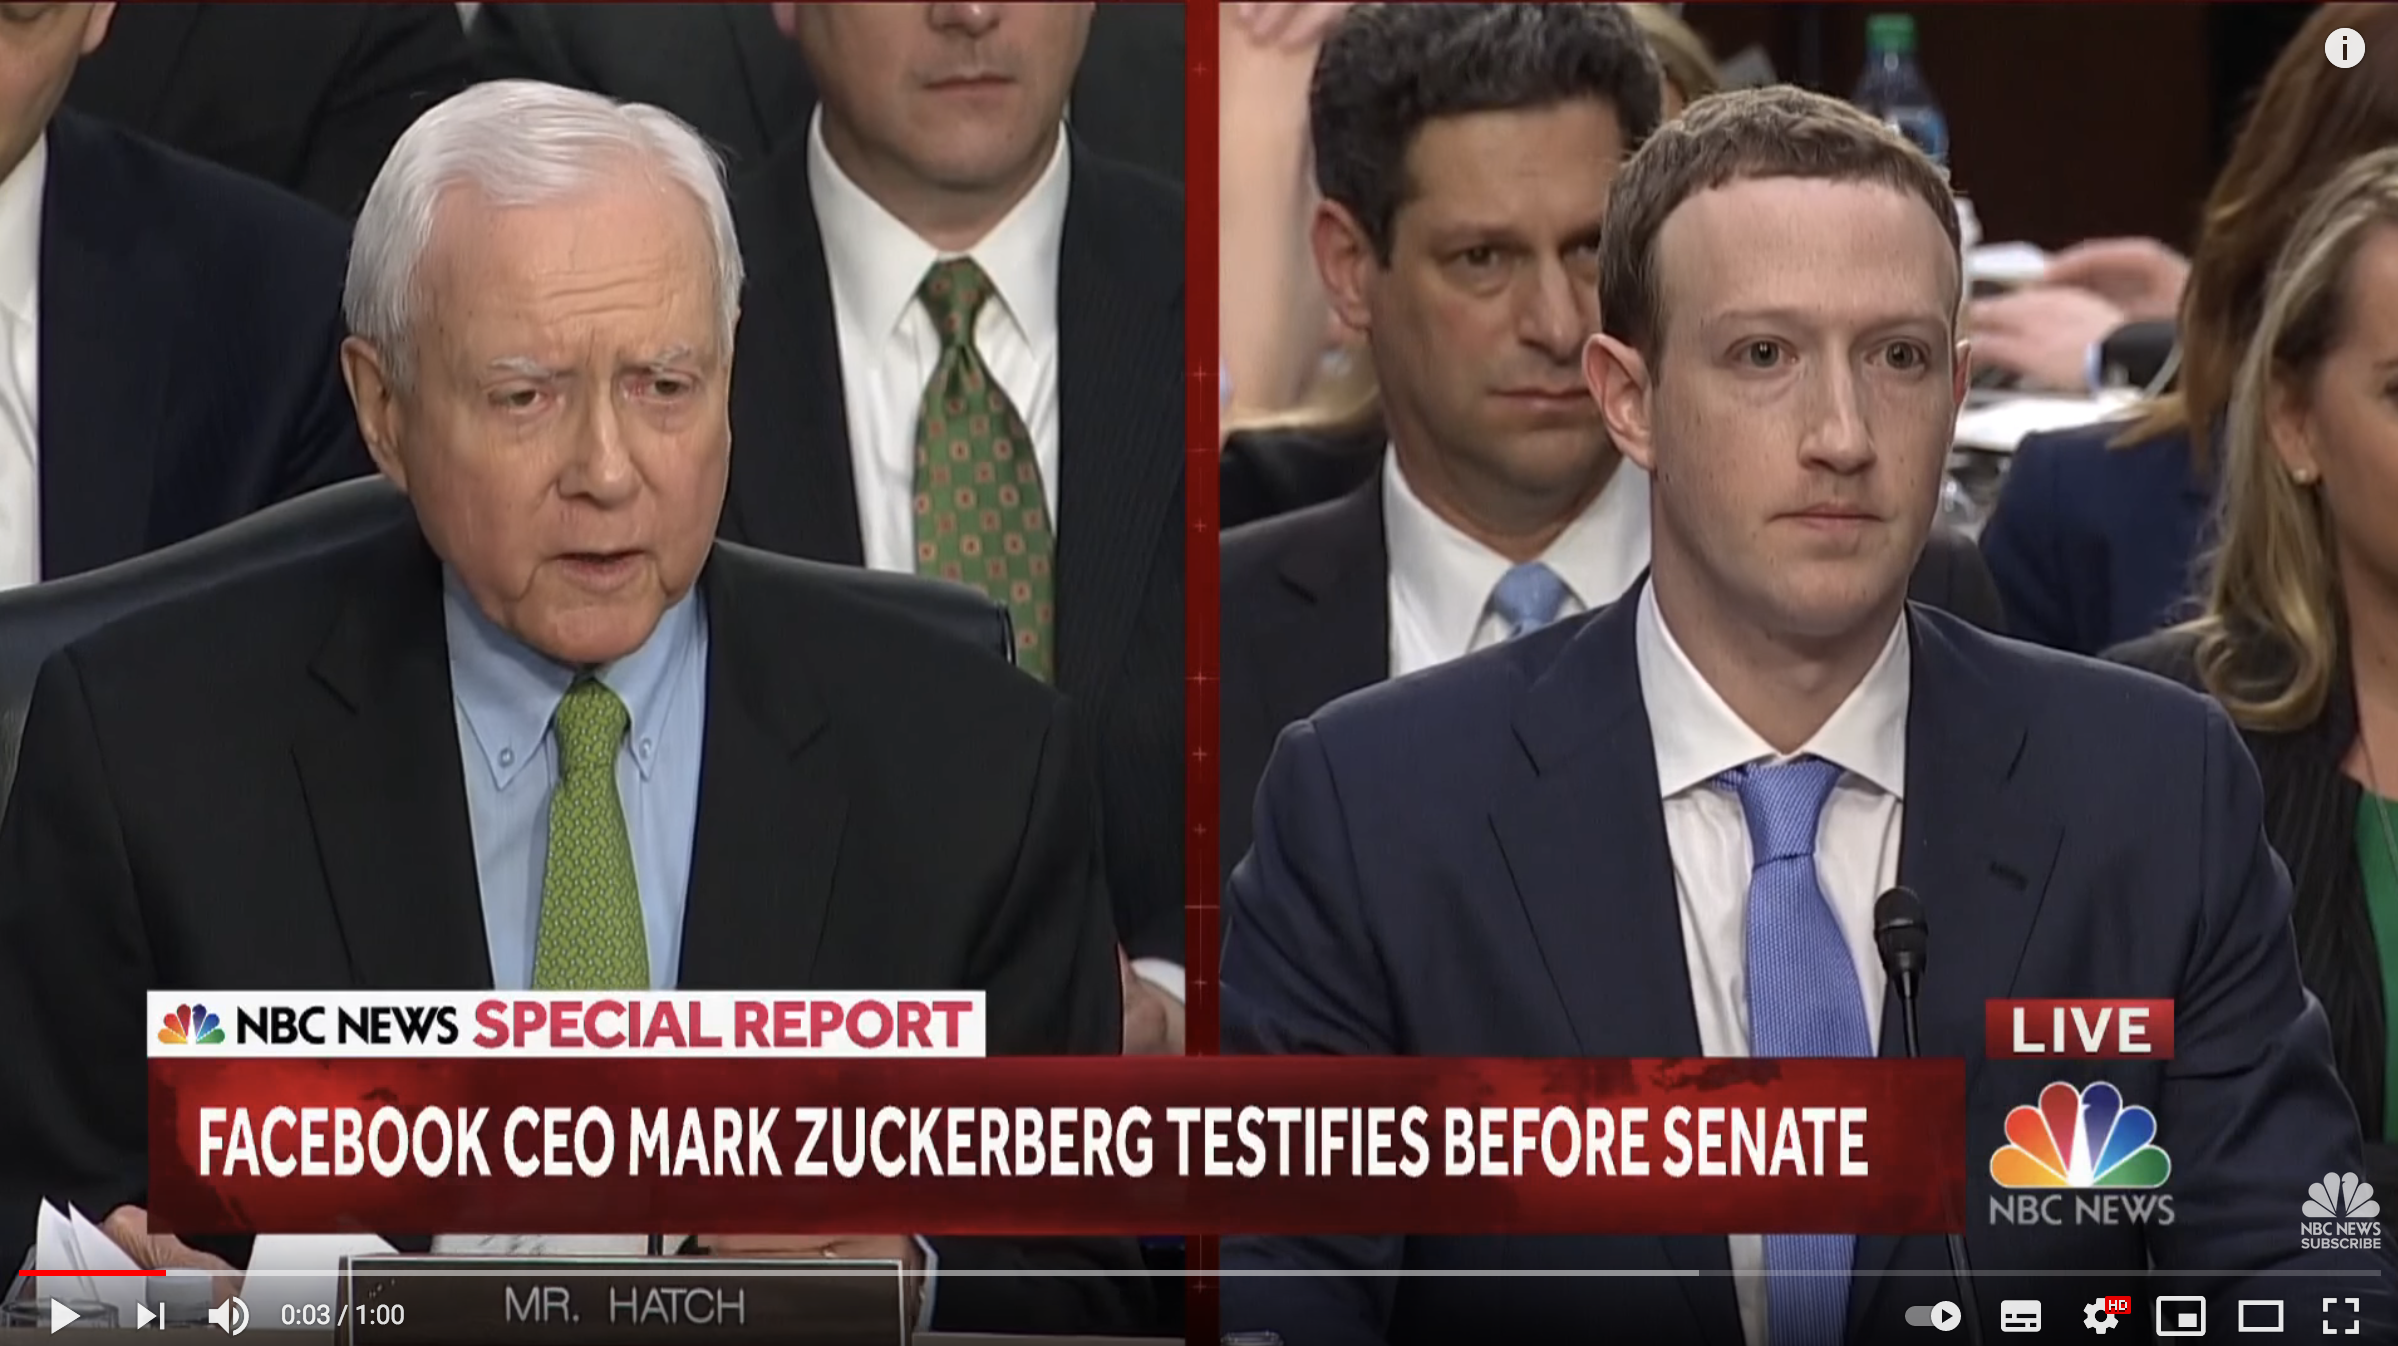
\includegraphics[width=0.9\textwidth]{figures/zuck_congress_video}
\end{center}

\vfill
\url{https://www.youtube.com/watch?v=n2H8wx1aBiQ}

\end{frame}
%%%%%%%%%%%%%%%%%%
\begin{frame}

Social media companies want to ``help connect everyone around the world and to bring the world closer together'' \pause and sell ads \pause that make lots and lots of money

\end{frame}
%%%%%%%%%%%%%%%%%
\begin{frame}

\begin{center}
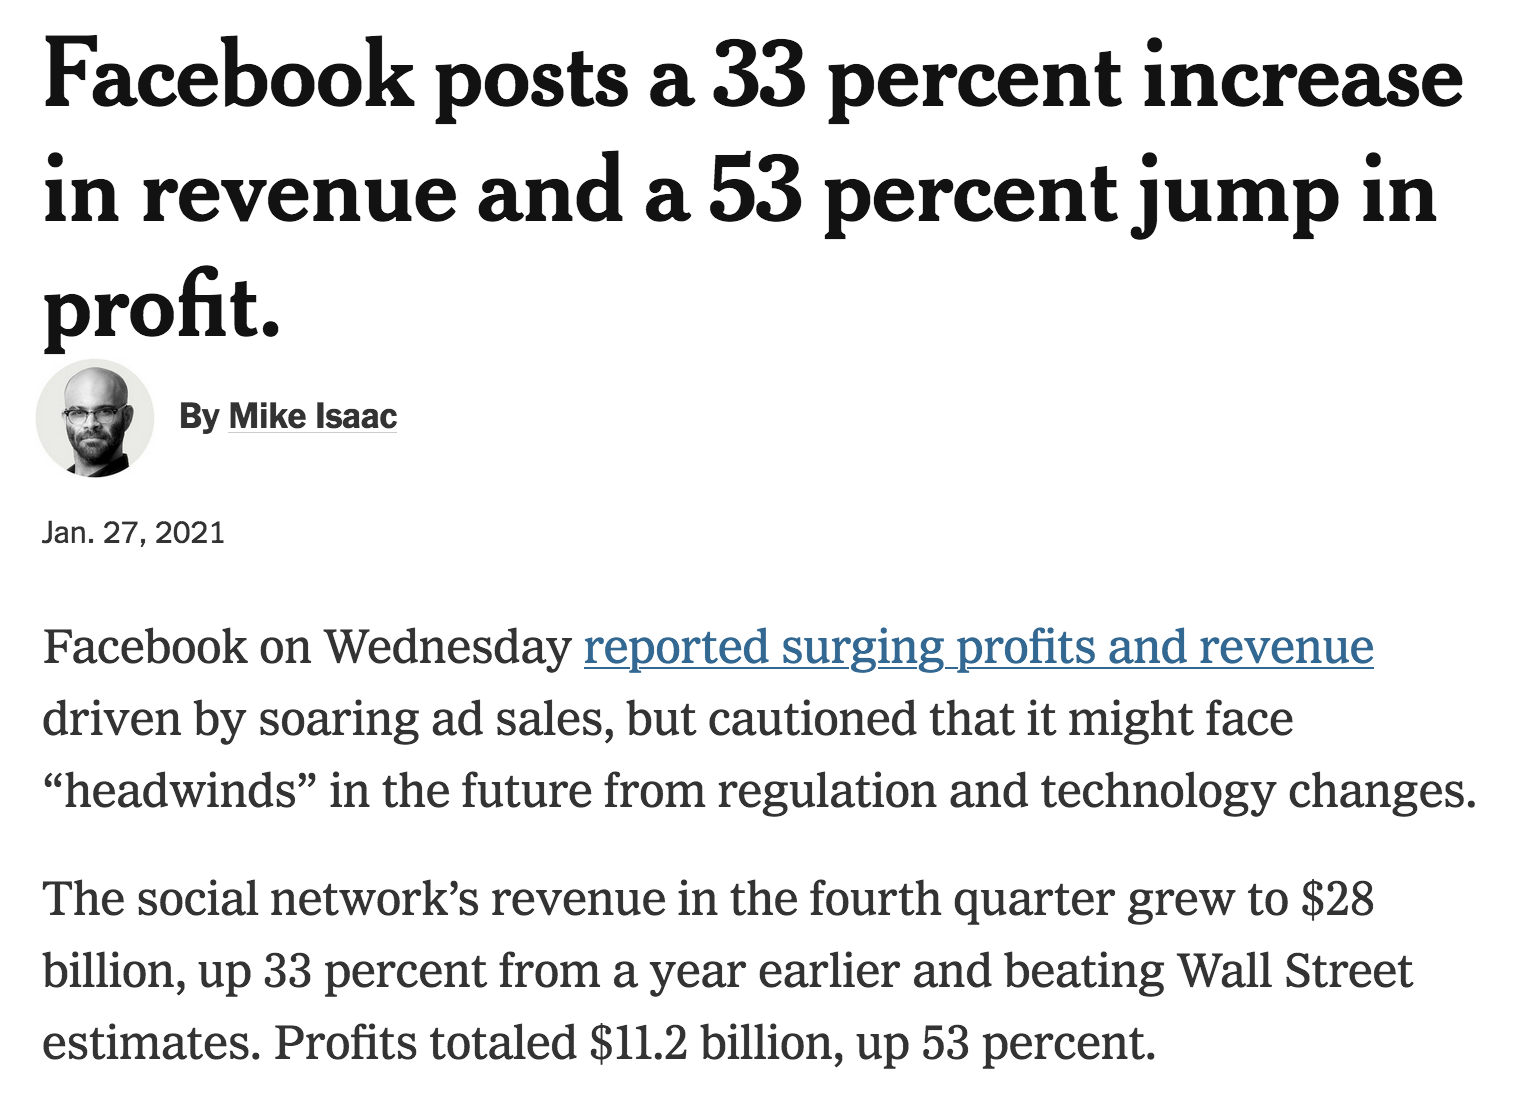
\includegraphics[width=0.7\textwidth]{figures/isaac_facebook_2021}
\end{center}

\vfill

\url{https://www.nytimes.com/2021/01/27/business/facebook-earnings.html}
\end{frame}
%%%%%%%%%%%%%%%%%
\begin{frame}

\begin{center}

\includegraphics[height=0.8\textheight]{figures/zuboff_age_2019_cover}
\end{center}

\vfill

Commodification of personal data for profit: \url{https://en.wikipedia.org/wiki/Surveillance_capitalism}

\end{frame}
%%%%%%%%%%%%%%%%%%
\begin{frame}

\begin{center}
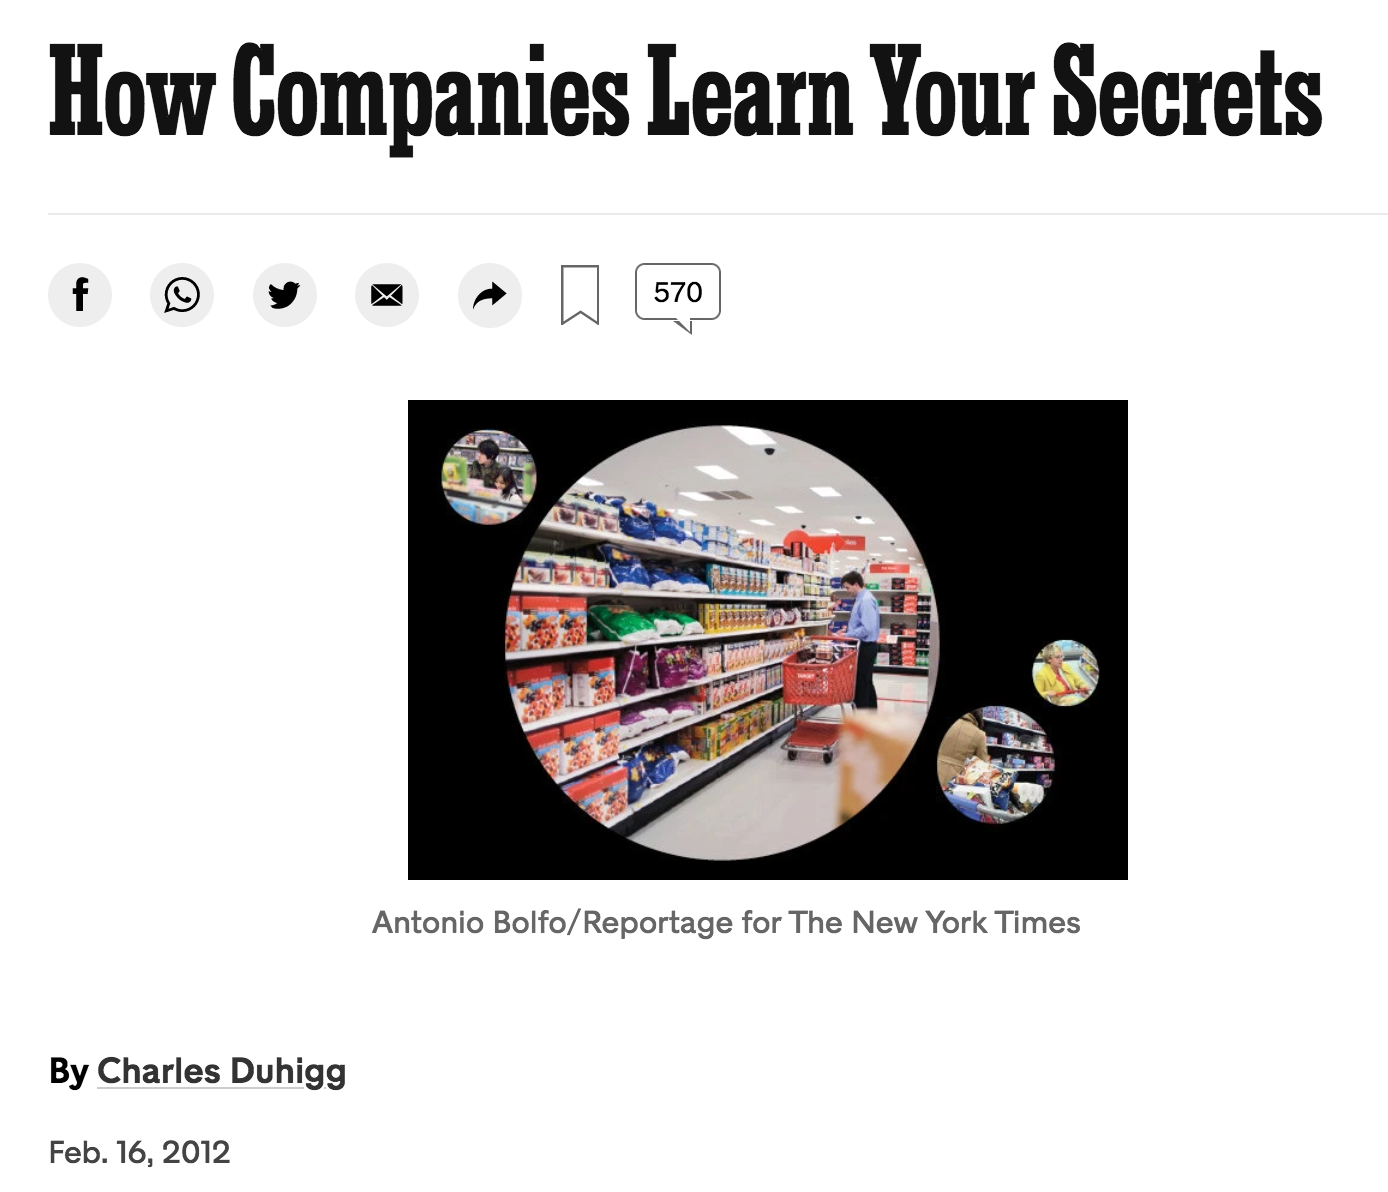
\includegraphics[height=0.8\textheight]{figures/duhigg_how_2012_top}
\end{center}

Pregnancy story illustrates surveillance capitalism, but Duhigg doesn't talk about social networks at all. 

\end{frame}
%%%%%%%%%%%%%%%%%%
\begin{frame}

"We regard social advertising as any advertising methods that uses information about consumers' social networks to target ads and/or provide personalized social signals.'' Bakshy et al.\

\begin{itemize}
\item Goel and Goldstein don't care about causality so they use observational data 
\item Bakshy et al.\ care about causality a lot so they run online field experiments
\item Both paper use the data from millions of people
\end{itemize}

\end{frame}
%%%%%%%%%%%%%%%%%%%
\begin{frame}

\begin{center}
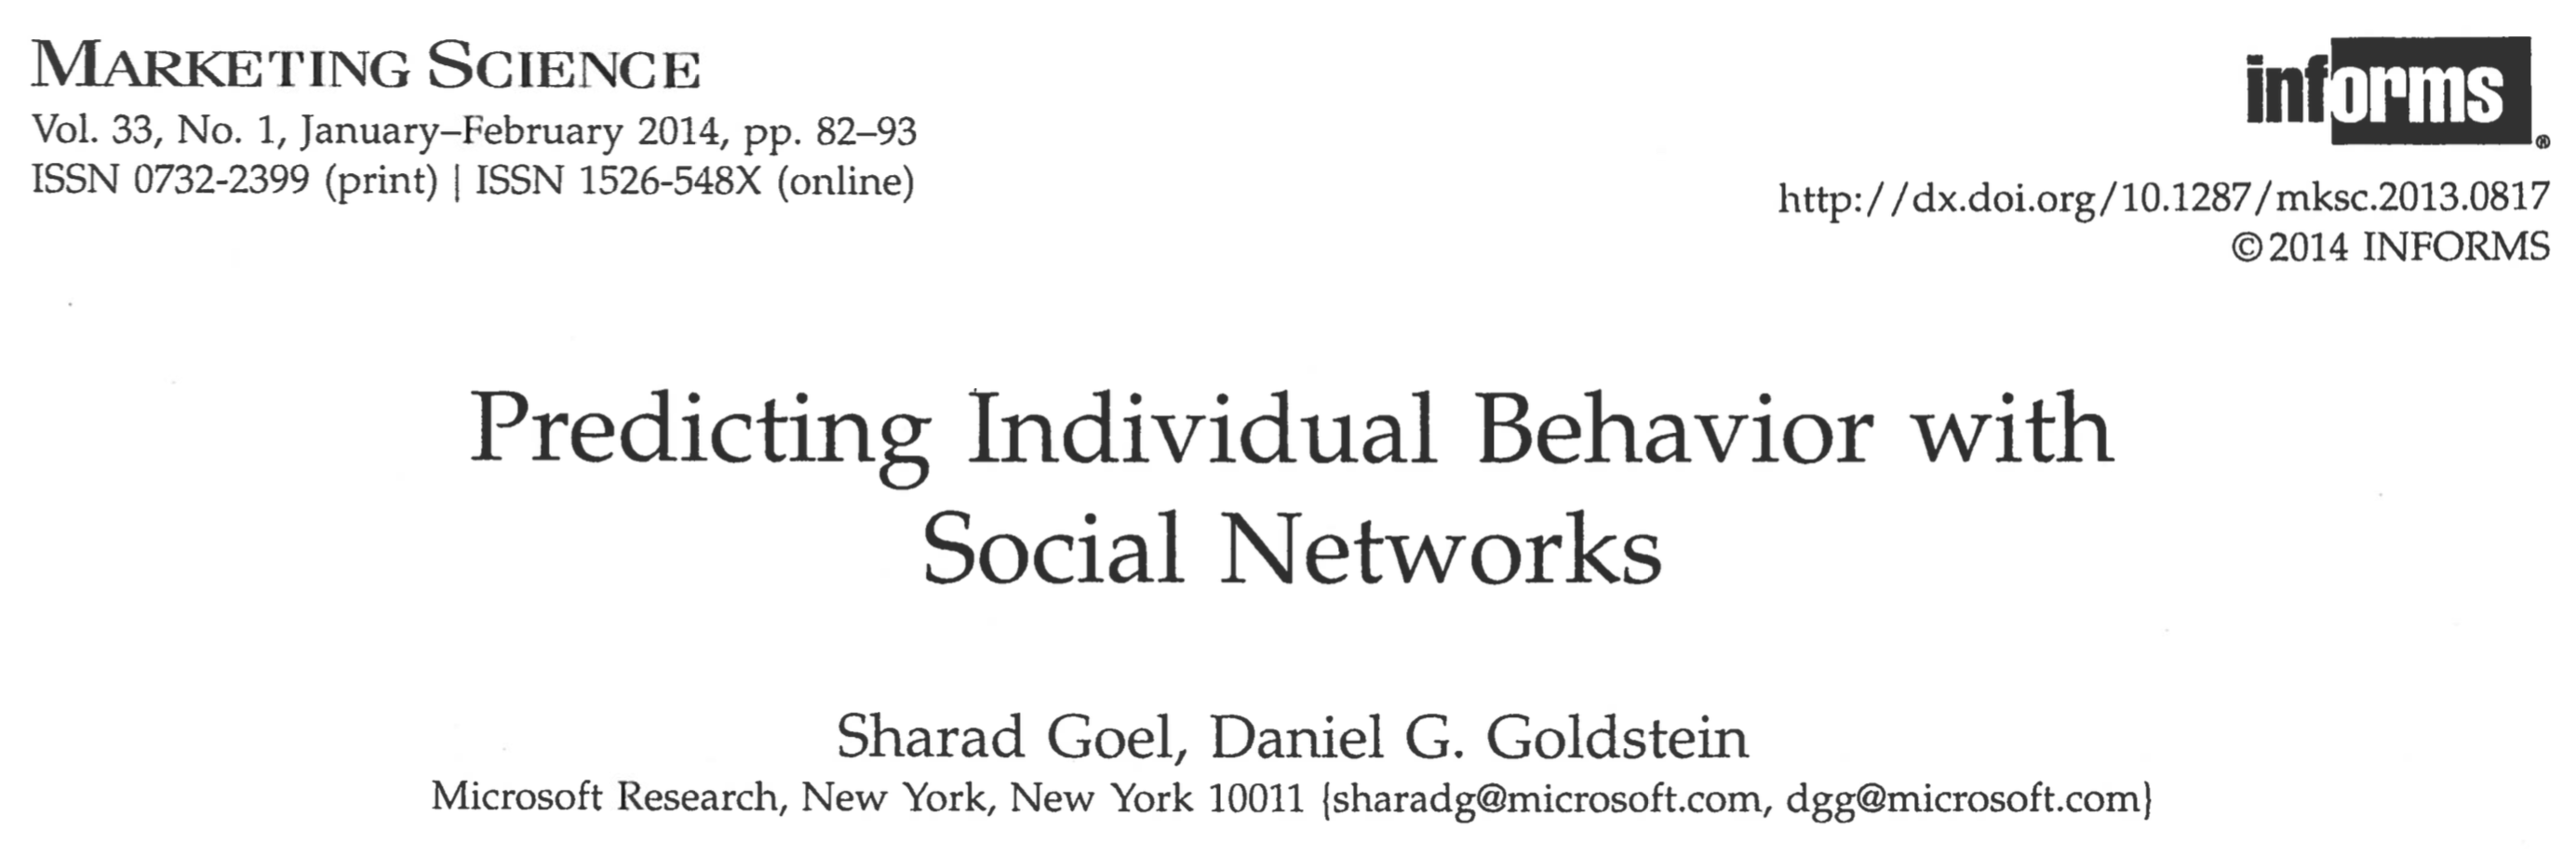
\includegraphics[width=\textwidth]{figures/goel_predicting_2014_title}
\end{center}

\begin{itemize}
\item Focus on managerially relevant question of assessing the worth of social network data for targeting and prediction \pause
\begin{itemize}
\item Does social network data help even in the presence of other data that companies already have (e.g., demographics and previous behavior)?
\item How many targets can network data help find? \pause
\end{itemize}
\item Given their focus, they don't care about causality
\end{itemize}

\end{frame}
%%%%%%%%%%%%%%%%%%%%%
\begin{frame}

\begin{itemize}
\item Social data comes from Yahoo! communications network.
\item Edge between people who mutually exchanged email or instant messages during a fixed two-month period. 
\item 132 million people and 719 million edges, with a mean of 11 contacts per individual.
\end{itemize}

\end{frame}
%%%%%%%%%%%%%%%%%%%%
\begin{frame}

\begin{center}
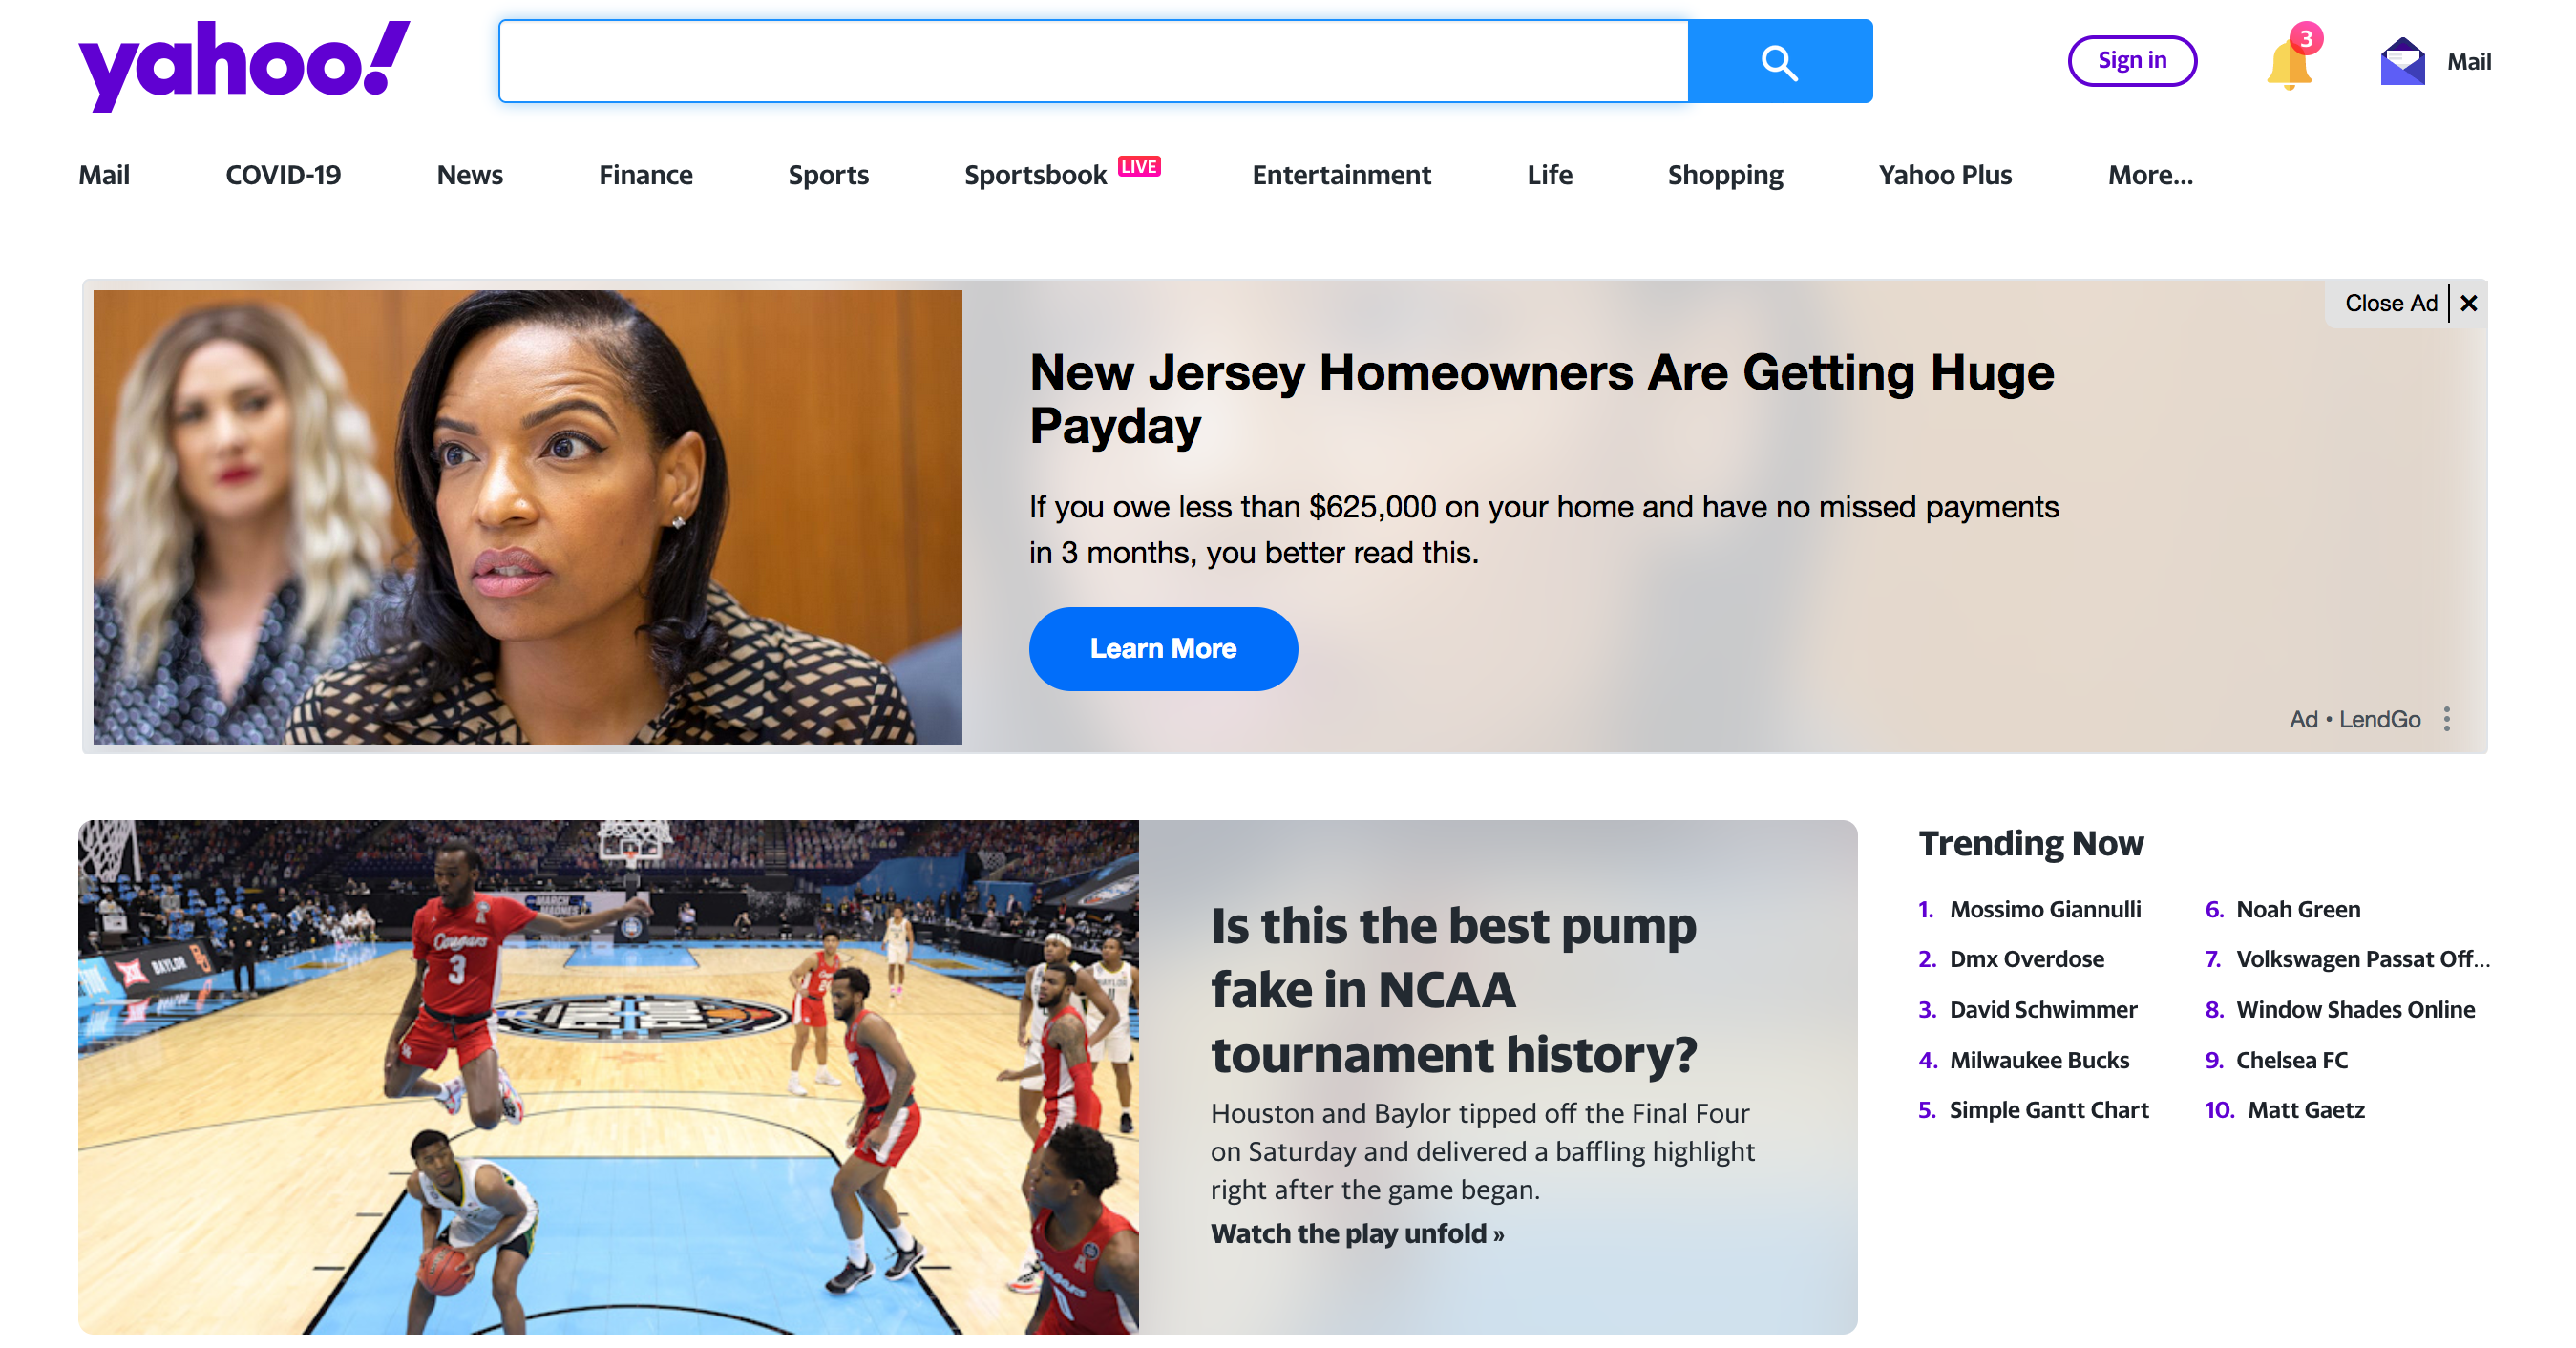
\includegraphics[width=\textwidth]{figures/yahoo_banner}
\end{center}

\note{
banner ads on yahoo}

\end{frame}
%%%%%%%%%%%%%%%%%%%%%%
\begin{frame}

\begin{center}
\only<1>{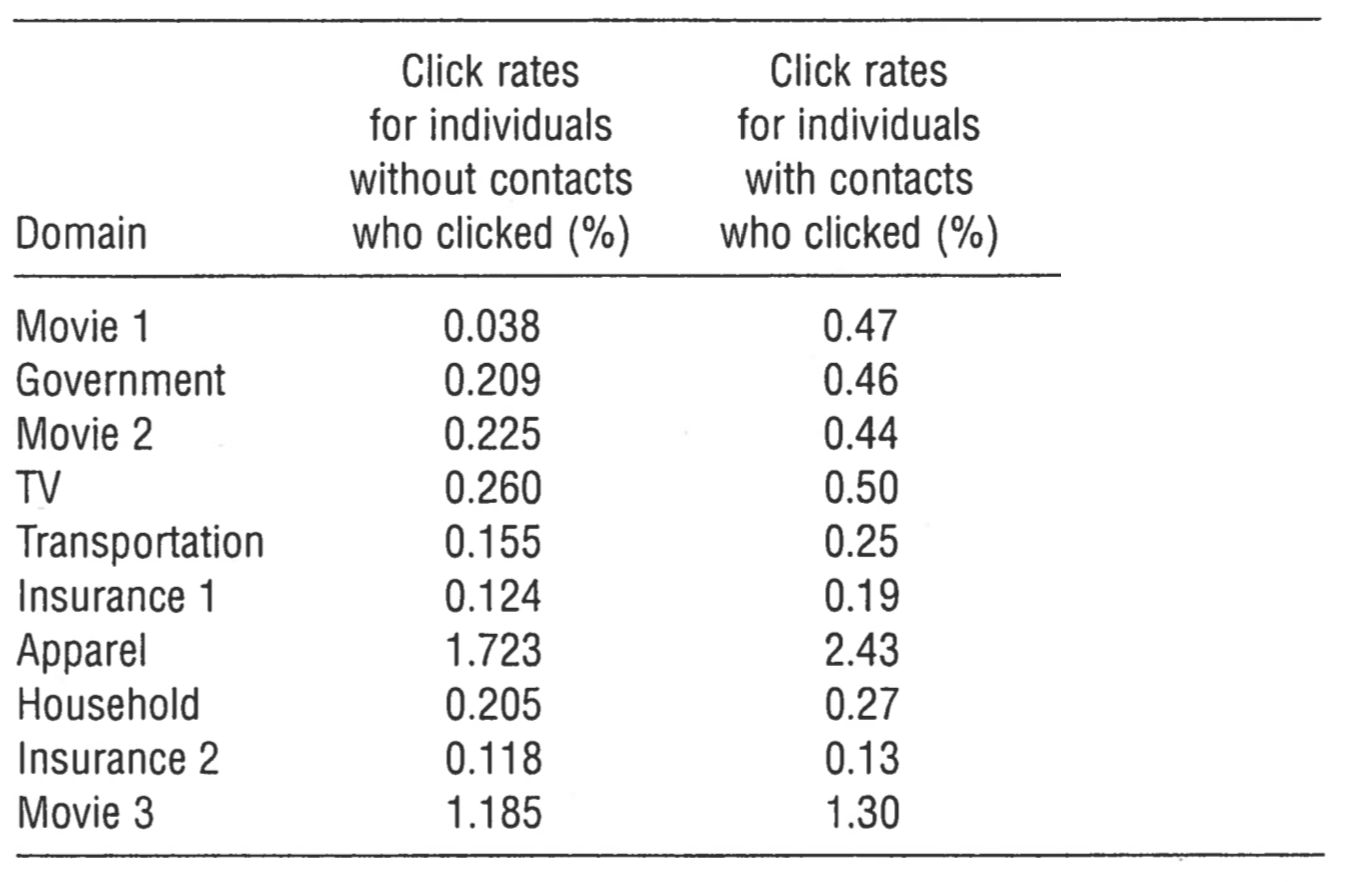
\includegraphics[width=0.5\textwidth]{figures/goel_predicting_2014_tab1_2columns}}
\only<2->{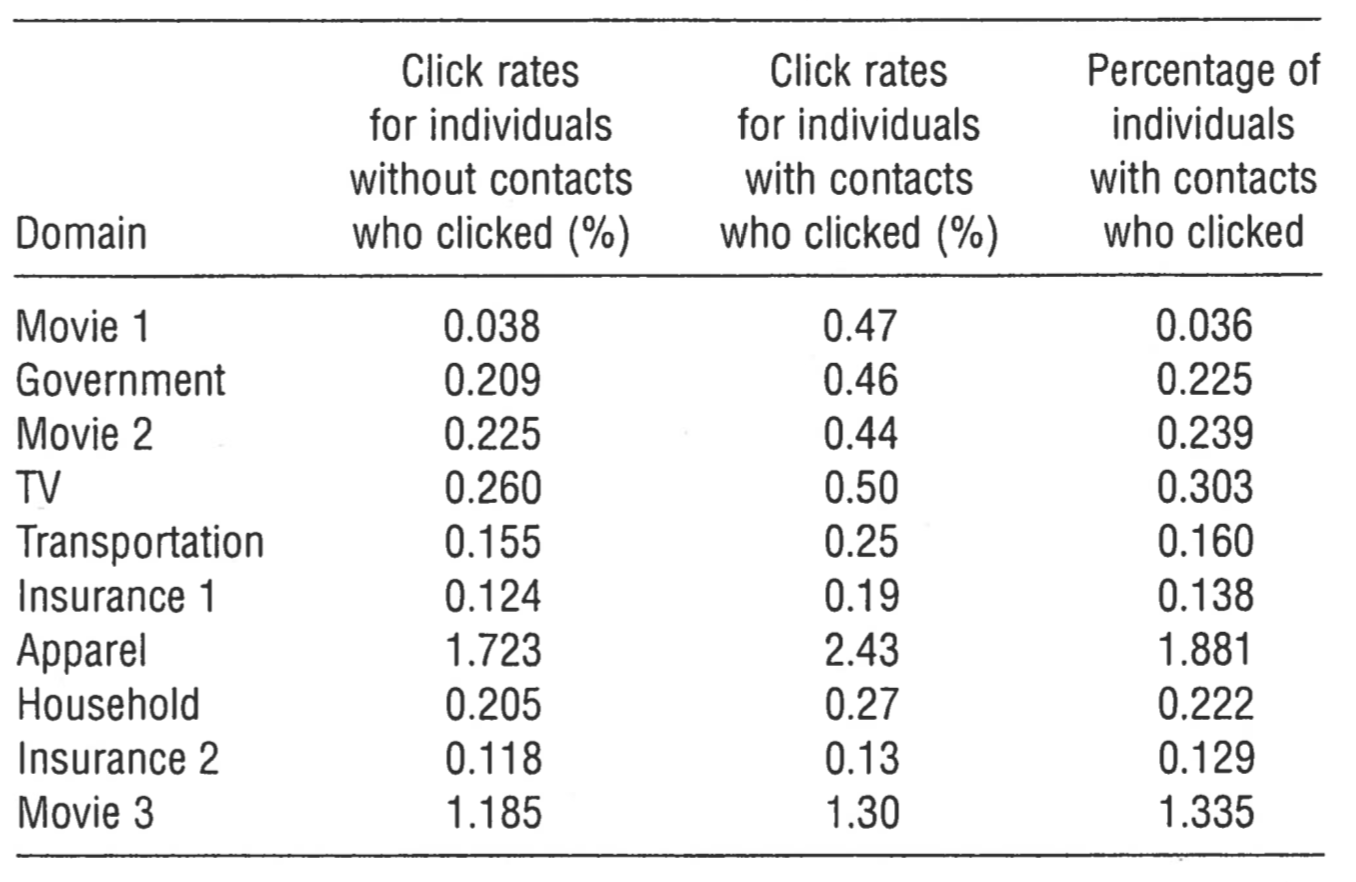
\includegraphics[width=0.5\textwidth]{figures/goel_predicting_2014_tab1}}
\end{center}
\vfill

\begin{itemize}
\item People with contacts who clicked on the ad are much more likely to click on the ad (probably not causal).  Seems like a good chance to make some money. \pause
\item But. . . . very few people have contacts who clicked on the ads.
\end{itemize}

\end{frame}
%%%%%%%%%%%%%%%%%
\begin{frame}

\begin{center}
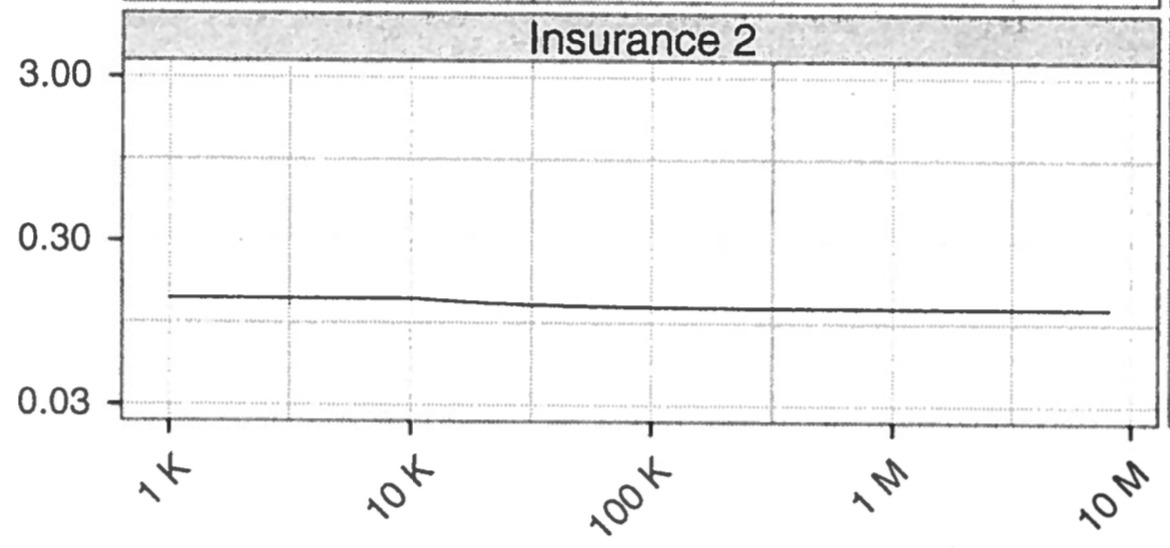
\includegraphics[width=\textwidth]{figures/goel_predicting_2014_fig1_insurance1}
\end{center}

\vfill
Top-k analysis: order people by the predicted probability of clicking, calculate predicted probability for different sized buckets of people

\end{frame}
%%%%%%%%%%%%%%%%%%
\begin{frame}

\begin{center}
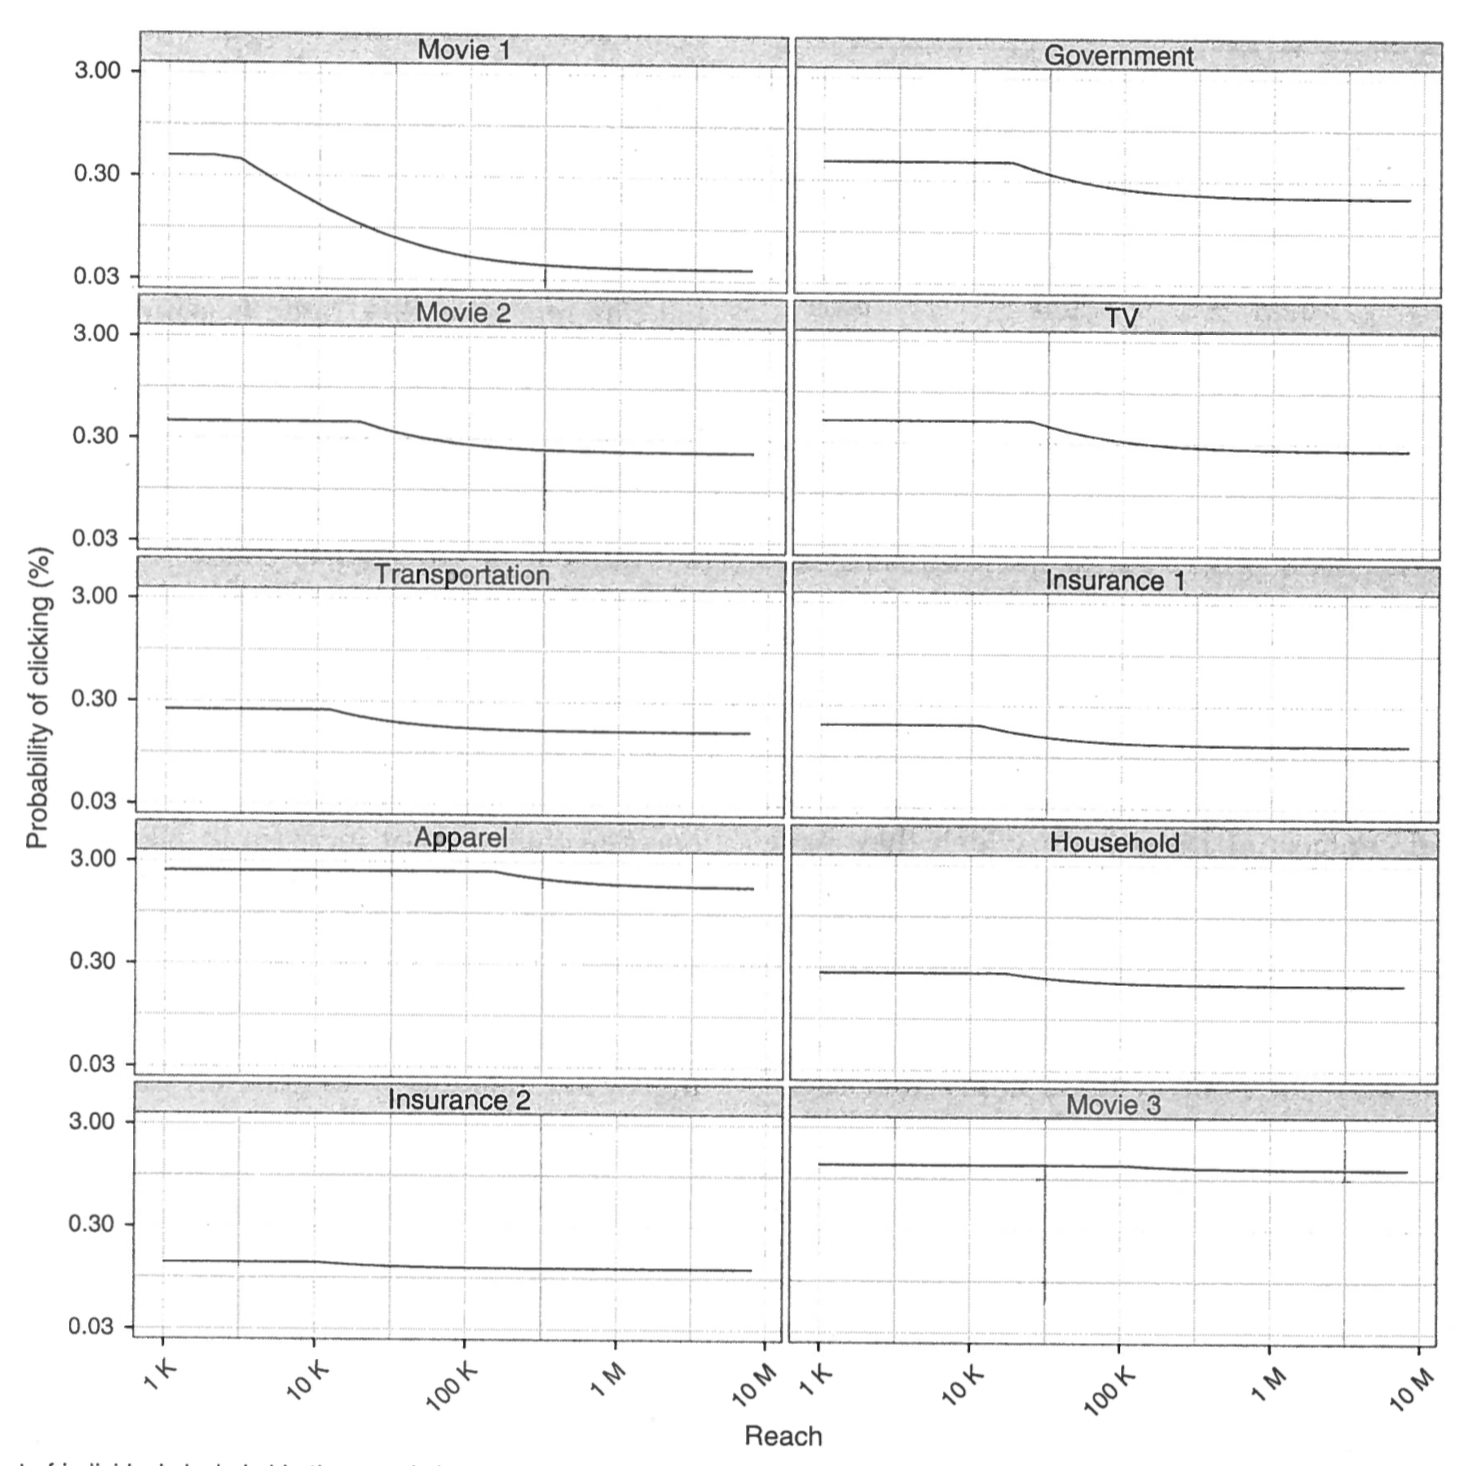
\includegraphics[height=0.8\textheight]{figures/goel_predicting_2014_fig1}
\end{center}

\vfill

\begin{itemize}
\item social signal allows you to construct pools of between 10,000 and 100,000 candidates who are more likely to click
\end{itemize}

\end{frame}
%%%%%%%%%%%%%%%%%%
\begin{frame}

\begin{center}
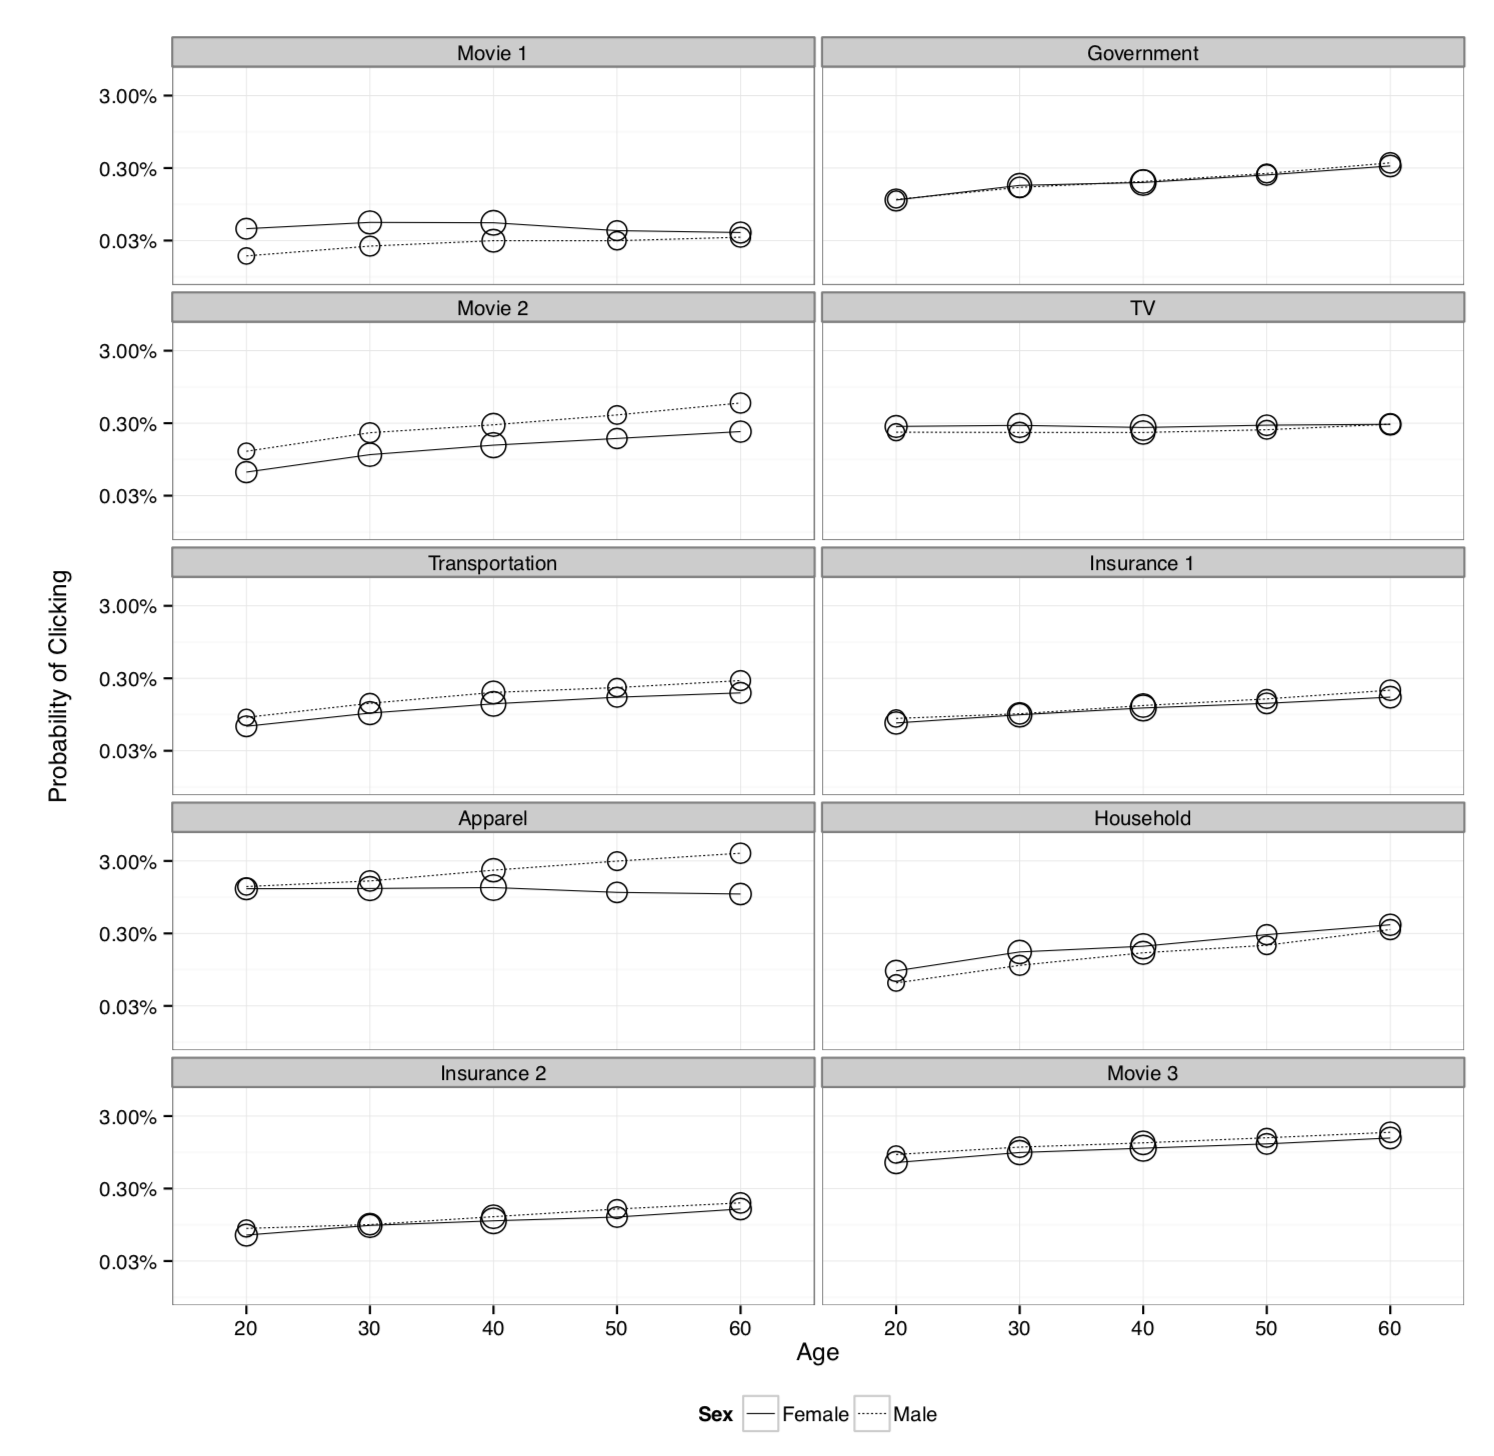
\includegraphics[height=0.6\textheight]{figures/goel_predicting_2014_figa2}
\end{center}

\vfill

\begin{itemize}
\item But there are important demographic differences as well. \pause
\item Does social add value even if you already have demographic data?
\end{itemize}

\end{frame}
%%%%%%%%%%%%%%%%%
\begin{frame}

\begin{center}
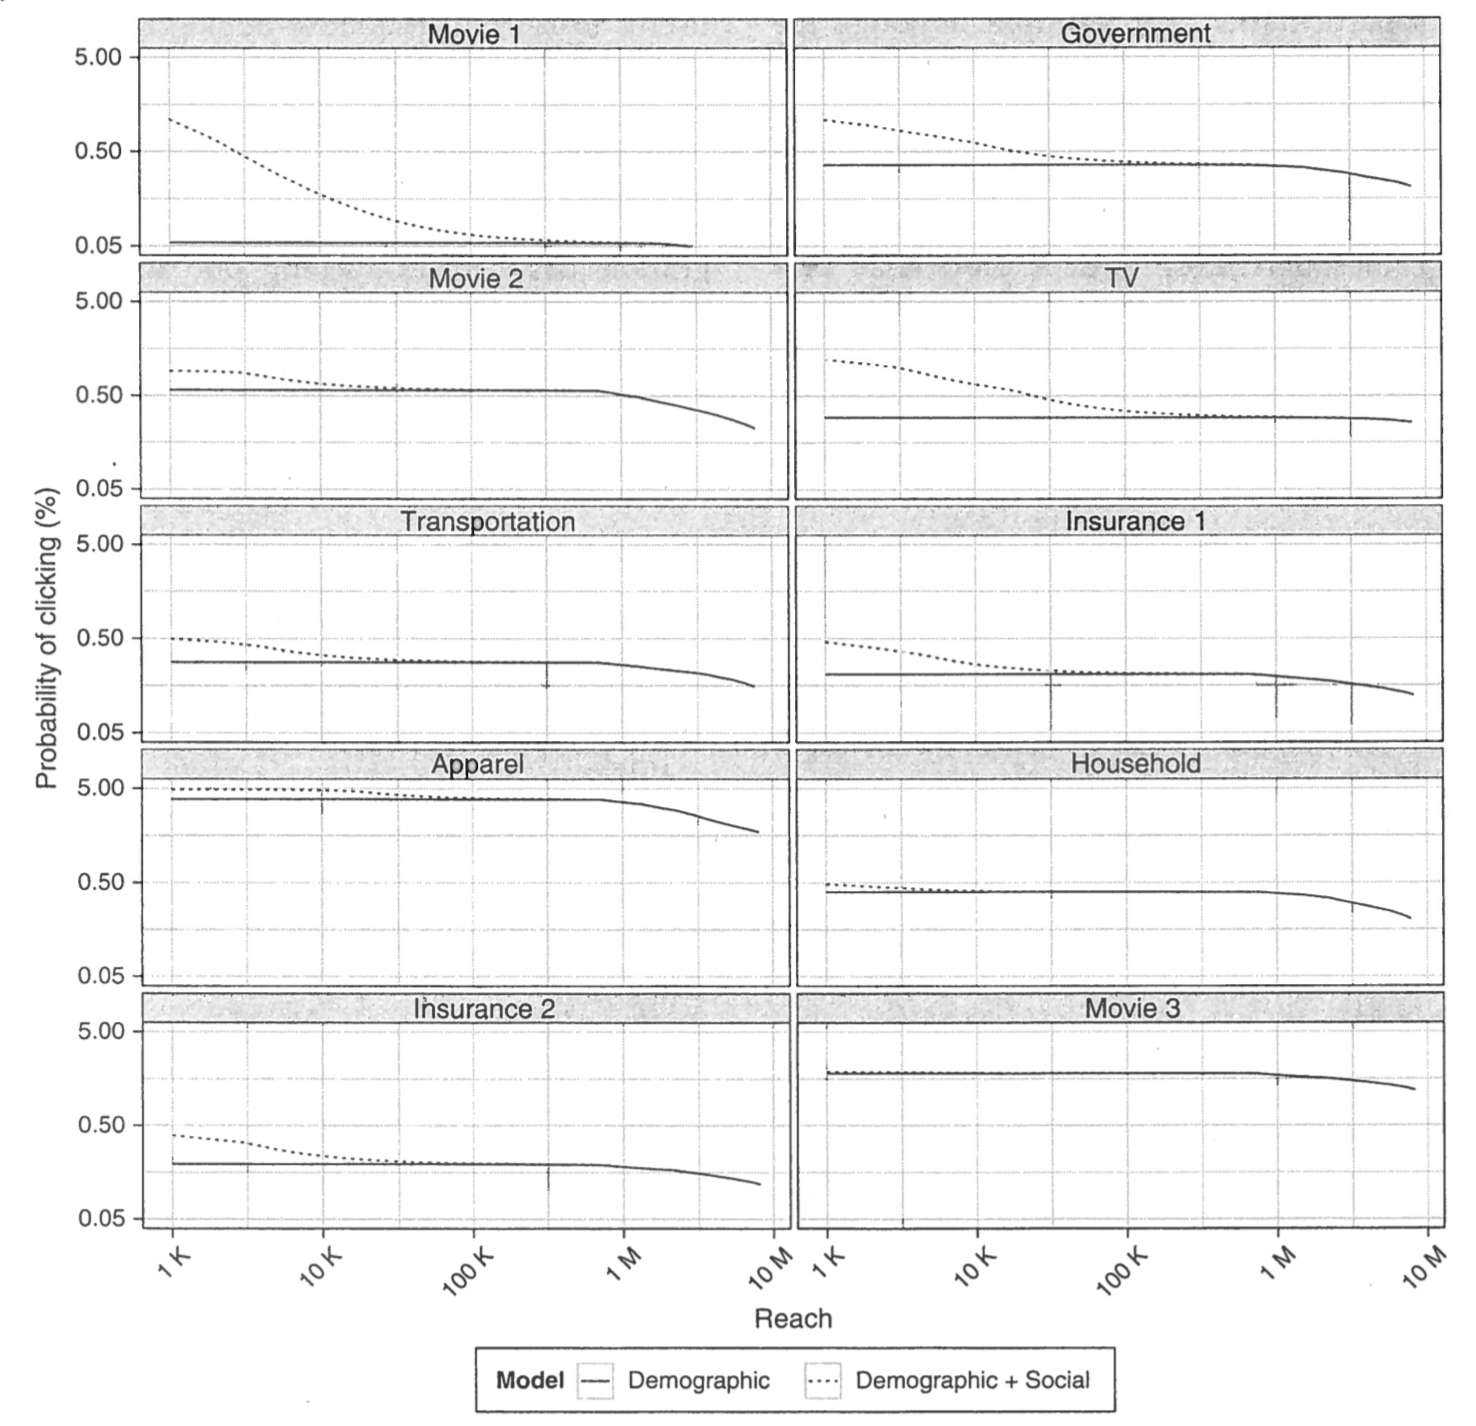
\includegraphics[height=0.6\textheight]{figures/goel_predicting_2014_fig2}
\end{center}

\vfill

\begin{itemize}
\item Demographic data alone can find large numbers of people who are more likely than average to click \pause
\item Even given that, social data since finds smaller groups more likely to click. But this group is small enough that it might not matter much.
\end{itemize}

\end{frame}
%%%%%%%%%%%%%%%%%
\begin{frame}

\setcounter{subfigure}{0}% Reset subfigure counter
\begin{figure}
  \centering
     \subfigure[Fantasy football]{
     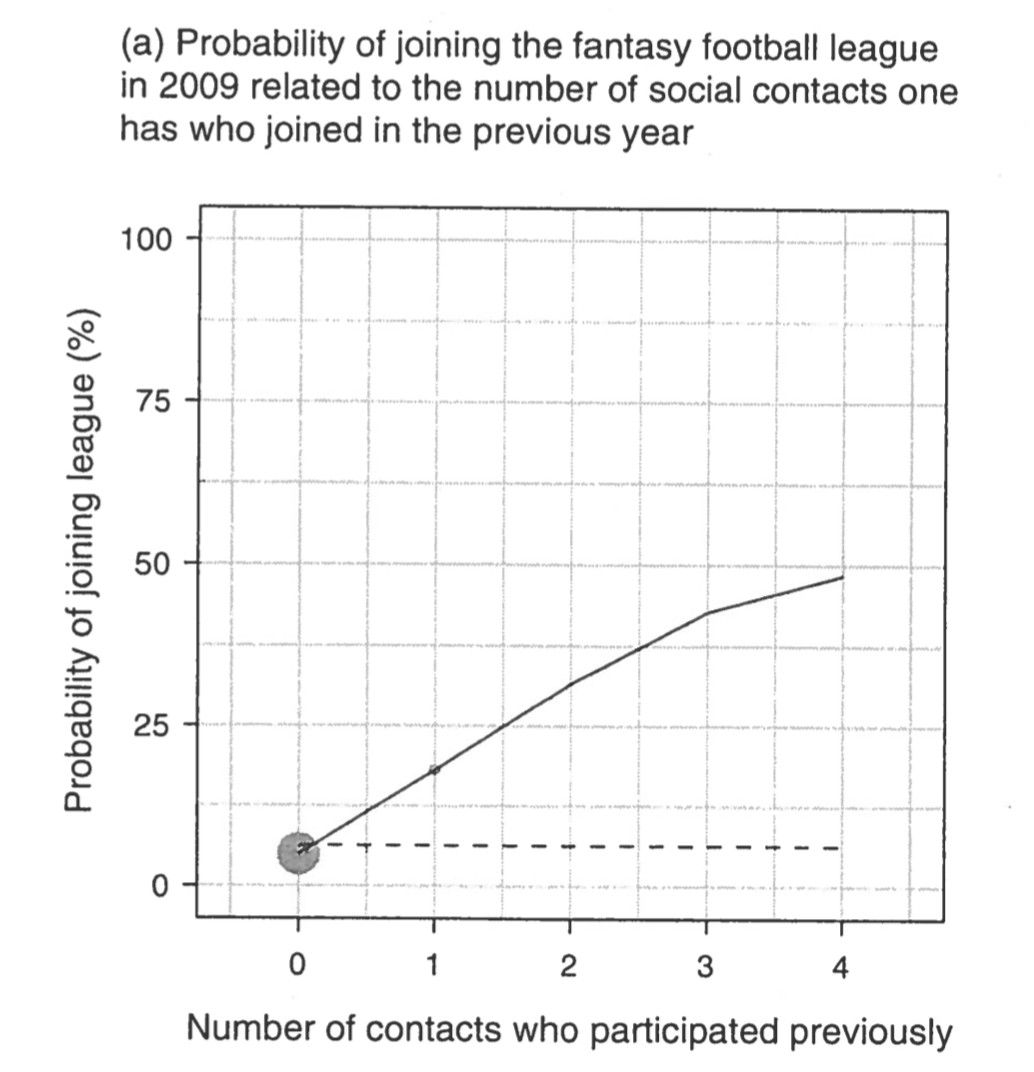
\includegraphics[width=0.40\textwidth]{figures/goel_predicting_2014_fig3a}}
  \hspace{0in}
  \subfigure[Retail purchase]{
     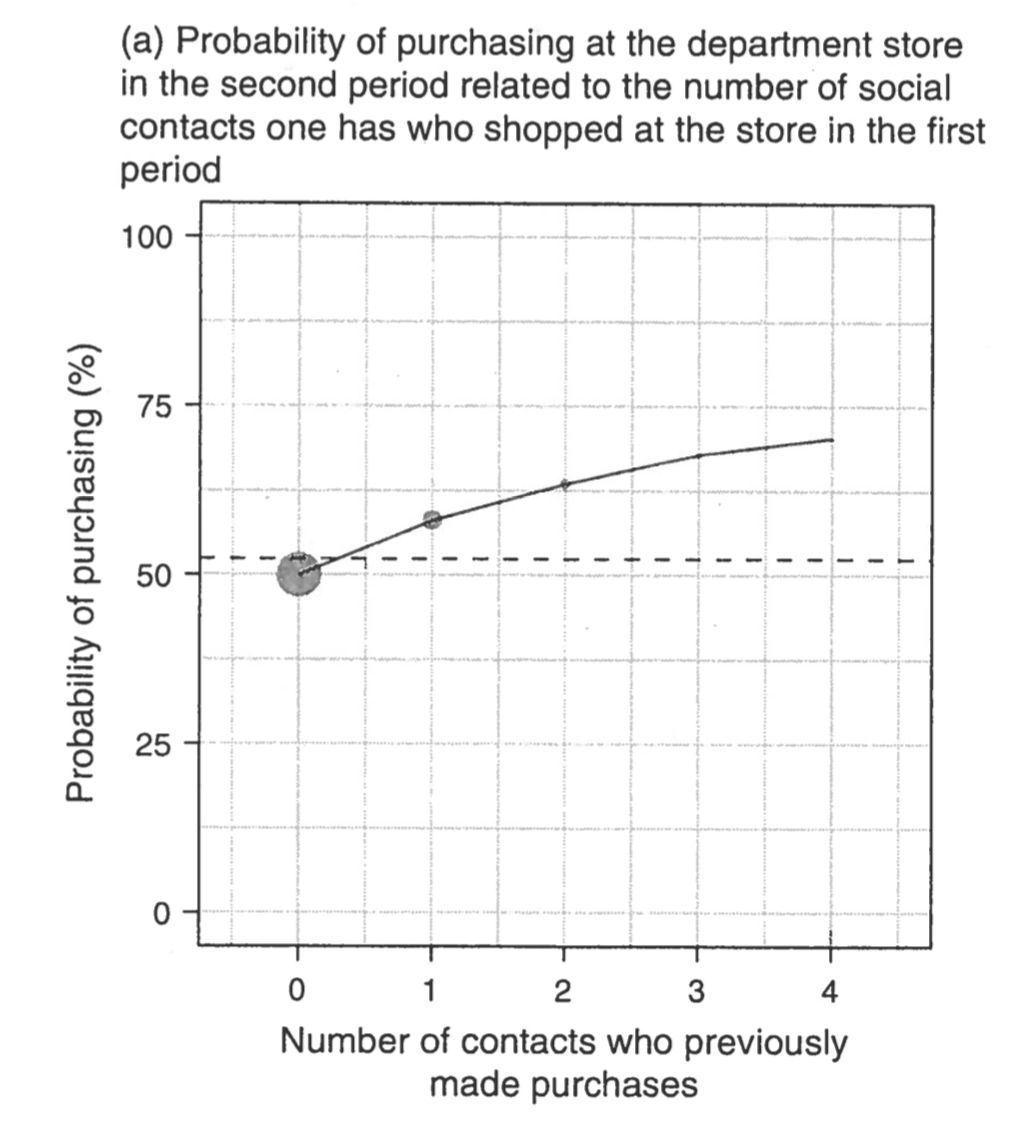
\includegraphics[width=0.40\textwidth]{figures/goel_predicting_2014_fig6a}}
\end{figure}

\vfill

\begin{itemize}
\item Probability of doing activity goes up with number of friends doing it but most people don't have friends going it
\end{itemize}

\end{frame}
%%%%%%%%%%%%%%%%%%
\begin{frame}

\setcounter{subfigure}{0}% Reset subfigure counter
\begin{figure}
  \centering
     \subfigure[Fantasy football]{
     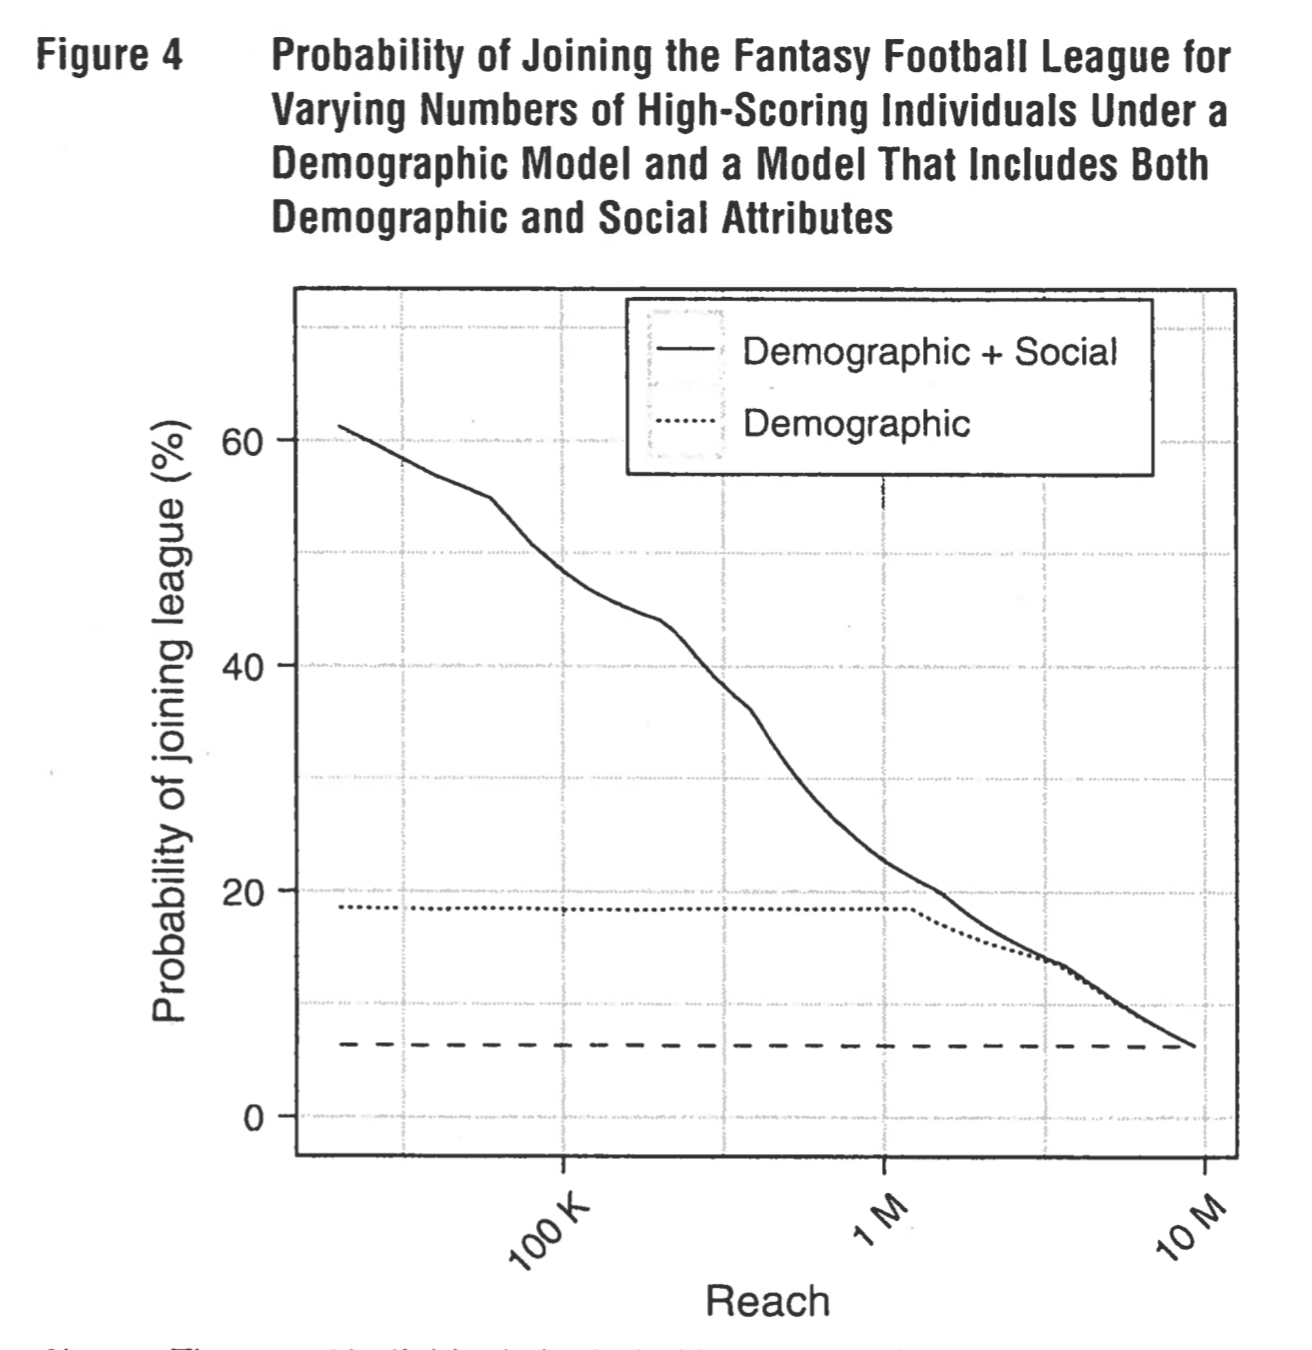
\includegraphics[width=0.45\textwidth]{figures/goel_predicting_2014_fig4}}
  \hspace{0in}
  \subfigure[Retail purchase]{
     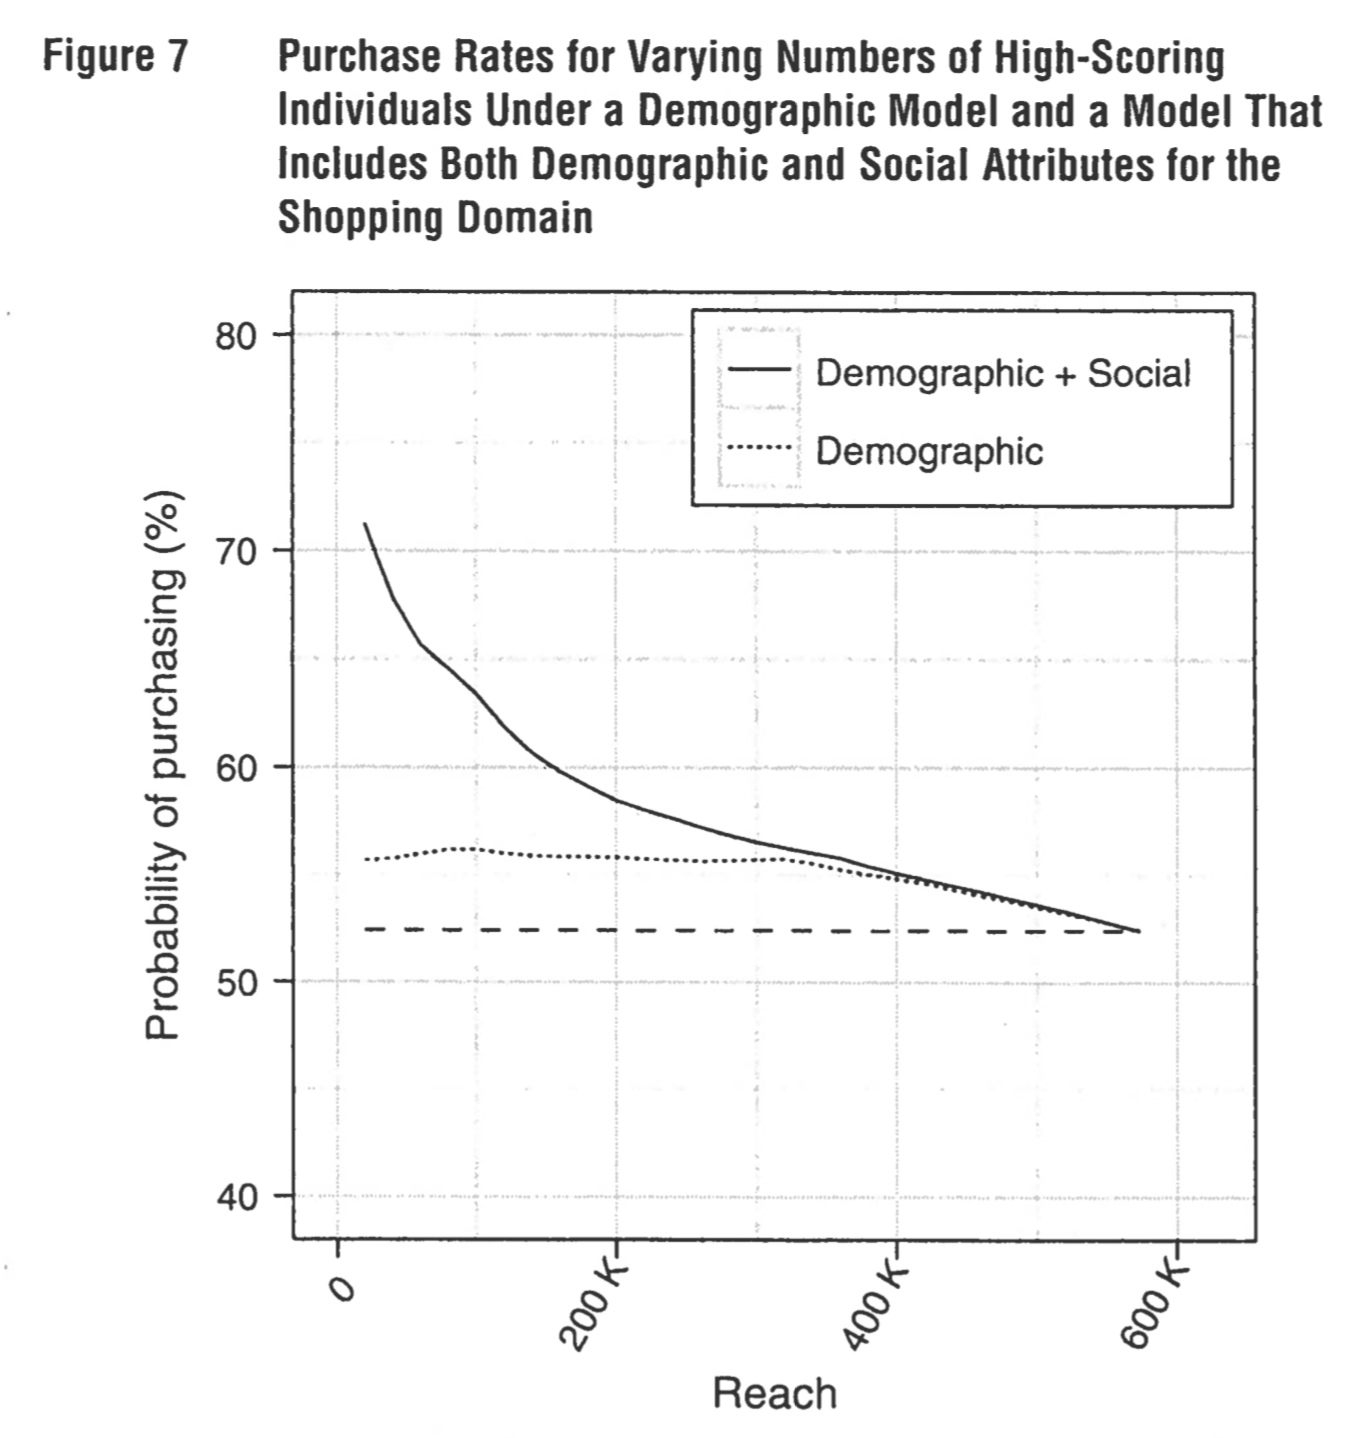
\includegraphics[width=0.45\textwidth]{figures/goel_predicting_2014_fig7}}
\end{figure}

\vfill
\begin{itemize}
\item Demographics beats baseline
\item Social + demographics beats demographics alone 
\end{itemize}

\end{frame}
%%%%%%%%%%%%%%%%%%
\begin{frame}

\begin{center}
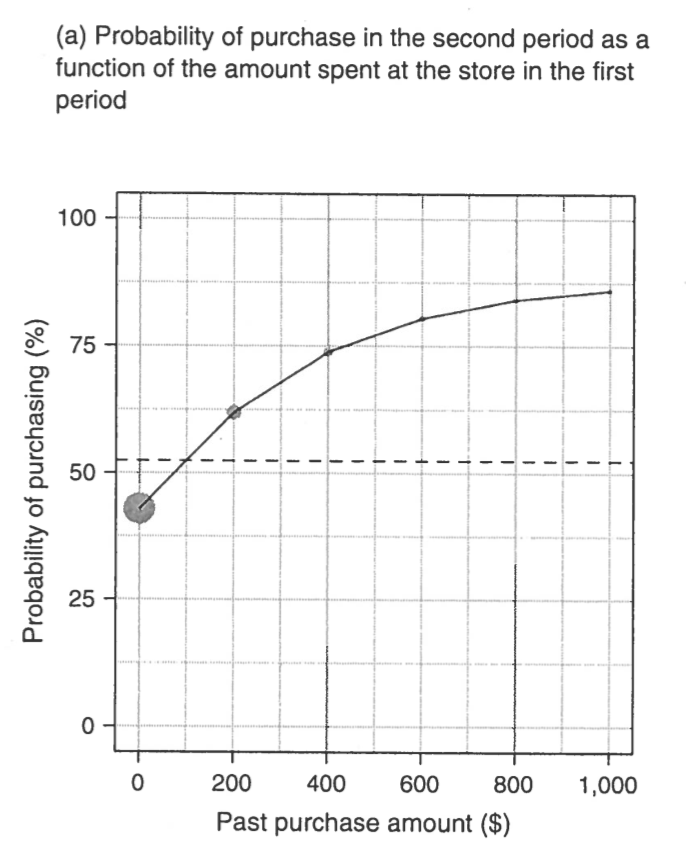
\includegraphics[height=0.8\textheight]{figures/goel_predicting_2014_fig8a}
\end{center}

\vfill

\begin{itemize}
\item People who spent more money in the past are more likely to purchase in next time period
\end{itemize}

\end{frame}
%%%%%%%%%%%%%%%%%
\begin{frame}

\begin{center}
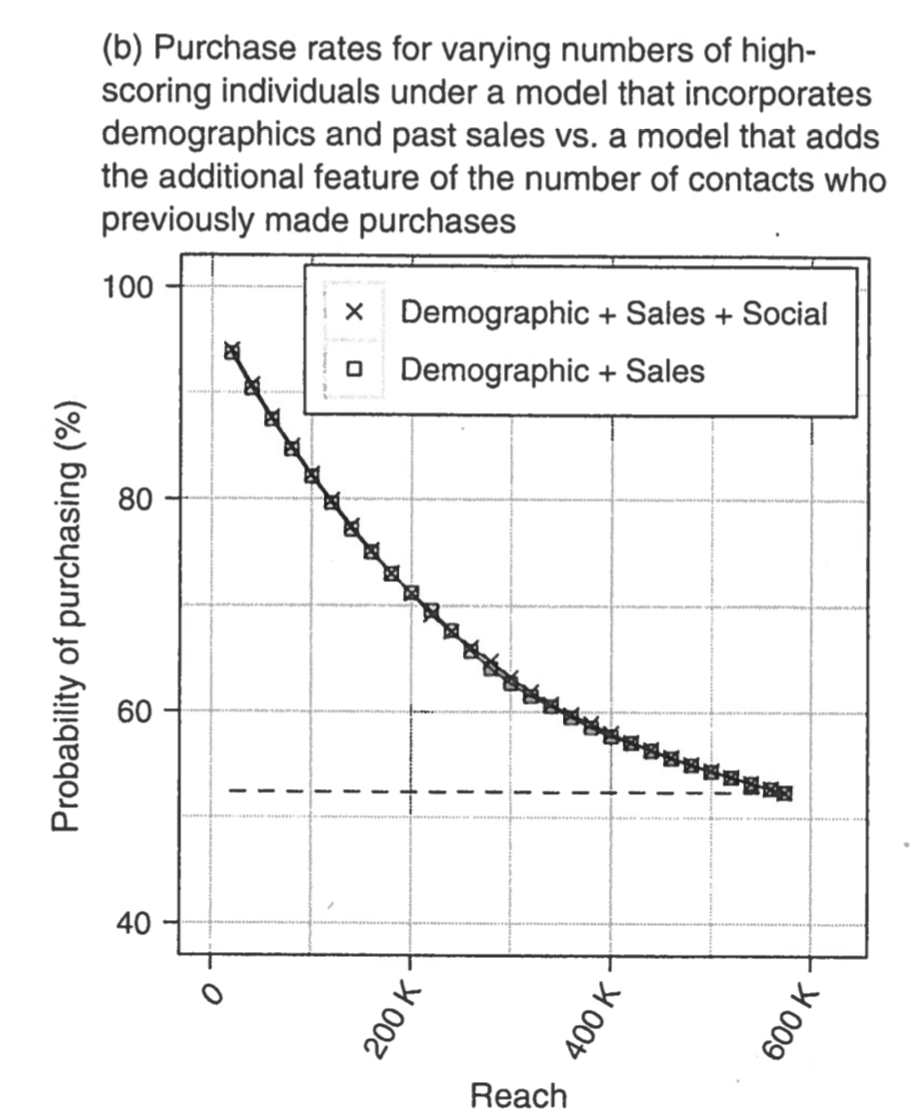
\includegraphics[height=0.8\textheight]{figures/goel_predicting_2014_fig8b}
\end{center}

\vfill

\begin{itemize}
\item Additional value of social is zero once model already has demographics and sales data
\end{itemize}

\end{frame}
%%%%%%%%%%%%%%%%%%%%%%
\begin{frame}

What about other ways that social data could be used?

\end{frame}

\end{document}
